\chapter{Planificación}

\label{cap:planificacion}


Después de aclarar los objetivos del proyecto y requisitos del mismo, es tiempo de realizar la planificación.\\

Para realizar la planificación del proyecto disponemos de múltiples alternativas, pero en este caso la técnica a usar son los diagramas de Gantt. Un diagrama de Grantt puede ser considerado una herramienta visual en la cual se ve reflejado el tiempo que va a ser empleado en cada una de las tareas del proyecto.\\

La planificación de este proyecto ha sido dividida en varios bloques que serán comentados a continuación:

\section{Primer acercamiento}

Este bloque ha sido dedicado a un estudio preliminar sobre nociones básicas de \textit{Android}, para garantizar que las bases del proyecto fuesen correctas y así asegurarse de partir de una buena base. Por otro lado, una vez terminado dicho estudio, se empleó el resto del tiempo en asegurar la posibilidad de elegir la imagen consulta usando la galería, o mediante la cámara del dispositivo, cosa que puede complicarse si no se realiza correctamente.

Como detalle, mencionar que mi experiencia con \textit{Android} era poca, por lo que este primer acercamiento ha sido de gran importancia, ya que ha sentado las bases del proyecto.

\begin{figure}[H] %con el [H] le obligamos a situar aquí la figura
\centering
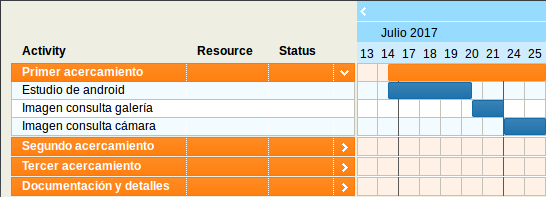
\includegraphics[scale=0.5]{imagenes/gant1.png}  %el parámetro scale permite agrandar o achicar la imagen. En el nombre de archivo puede especificar directorios
\label{gant1.png}
\caption{Diagrama Gantt. Primer acercamiento}
\end{figure}

El proyecto fue comenzado el 15 de julio. Los primeros días fueron empleados en el estudio de \textit{Android}, punto fundamental para empezar el proyecto. El resto de días se usaron para posibilitar la elección de la imagen consulta a través de la cámara o galería, gestionando los permisos de una forma adecuada.

\section{Segundo acercamiento}

Una vez establecido el punto de partida e instalado todo lo necesario pasamos al segundo bloque.\\

En este bloque se realizó un análisis para establecer cuales eran los requisitos necesarios para el correcto funcionamiento del proyecto.
Por otro lado, se desarrolló una interfaz prototipo, en la cual era posible seleccionar la imagen consulta, como hemos comentado anteriormente. Las imágenes consulta se mostraban en la parte superior de la pantalla, mientras que las imágenes resultado se mostraban en la parte inferior.\\

También se desarrolló un descriptor prototipo, para comprobar que realmente podíamos trabajar bien con las imágenes en \textit{Android}. Dicho descriptor únicamente cogía los píxeles de las imágenes y hacía cálculos triviales. Con esto, se estableció la estructura que debían tener los descriptores que se implementaron en el siguiente bloque.

\begin{figure}[H] %con el [H] le obligamos a situar aquí la figura
\centering
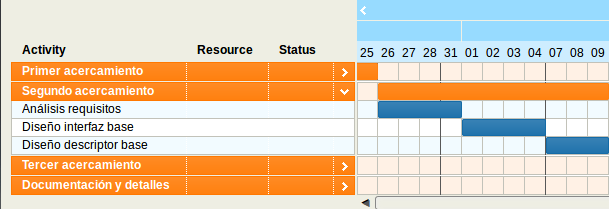
\includegraphics[scale=0.5]{imagenes/gant2.png}  %el parámetro scale permite agrandar o achicar la imagen. En el nombre de archivo puede especificar directorios
\label{gant2.png}
\caption{Diagrama Gantt. Segundo acercamiento}
\end{figure}

En este bloque el tiempo ha sido repartido de manera casi equitativa entre el análisis de requisitos, el diseño de la interfaz prototipo y del descriptor prototipo. Cosa crucial para la correcta realización del proyecto, ya que, aparte de implementar los prototipos, todos los requisitos deben estar establecidos antes de avanzar en el proyecto.\\

\section{Tercer acercamiento}

Este es el bloque al cual se le ha dedicado más tiempo en este proyecto, debido a que es en el que se ha procedido a la implementación de la interfaz final, de los descriptores y de la base de datos.\\

La interfaz sigue un estilo similar a la prototipo, con las imágenes consulta en la parte superior y en la inferior las imágenes resultado de la consulta. A su vez cuenta con otros apartados como ajustes e información adicional. Todo esto se comentará con detalle en su correspondiente sección.\\

Por el momento se han implementando dos descriptores:
\begin{itemize}
\item Media de color
\item Color estructurado
\end{itemize}

El primero se basa en el color medio de las imágenes, mientras que el segundo utiliza el histograma. Como en el caso de la interfaz, esto se detallará con más detalle.\\

Finalmente, después de todo lo anterior se decidió a implementar una pequeña base de datos que almacenase los valores obtenidos durante las consultas, de esta manera, en lugar de calcular el color medio o el histograma, se consultará en la base de datos y se obtendrá su valor, lo que reduce el tiempo de consulta drásticamente.\\

\begin{figure}[H] %con el [H] le obligamos a situar aquí la figura
\centering
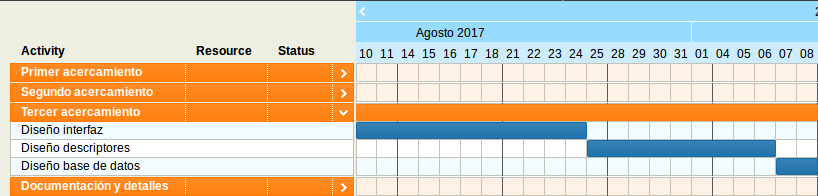
\includegraphics[scale=0.5]{imagenes/gant3.png}  %el parámetro scale permite agrandar o achicar la imagen. En el nombre de archivo puede especificar directorios
\label{gant3.png}
\caption{Diagrama Gantt. Tercer acercamiento}
\end{figure}


\section{Documentación y detalles}

En este último bloque se ha procedido a la realización de esta memoria y a su vez a la revisión de todo el proyecto en busca de erratas y malfuncionamiento.\\

\begin{figure}[H] %con el [H] le obligamos a situar aquí la figura
\centering
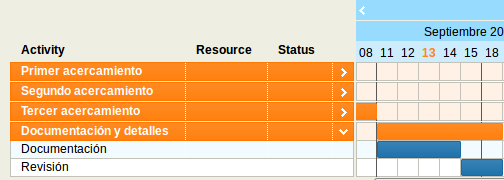
\includegraphics[scale=0.5]{imagenes/gant4.png}  %el parámetro scale permite agrandar o achicar la imagen. En el nombre de archivo puede especificar directorios
\label{gant4.png}
\caption{Diagrama Gantt. Documentación y detalles}
\end{figure}

Tras terminar todo el proyecto es muy importante revisarlo minuciosamente con el objetivo de encontrar fallos o elementos que se encuentren mal explicados. Por eso este bloque es gran importancia a pesar de ser el último.
